\documentclass[../../InformazioneQuantistica.tex]{subfiles}

\begin{document}

%\section{Algoritmo di Grover - parte 2}
Partiamo dallo stato iniziale:
\begin{align*}
\ket{\Psi_0} &= \ket{00}_{12}\ket{1}_3
\intertext{dove i primi $2$ qubit codificano il primo indice del database, e il terzo è un \textit{qubit ancilla} necessario per la computazione reversibile.}
\intertext{Analogamente a quanto visto per l'algoritmo di Deutsch, applichiamo ad ogni qubit un gate Hadamard per realizzare una sovrapposizione di tutti gli stati possibili, giungendo a:}
\ket{\Psi_1} &= H^{\otimes 3} \ket{\Psi_0} = \frac{1}{2}\Big[\ket{00}+\ket{01}+\ket{10}+\ket{11}\Big]_{12} \frac{1}{\sqrt{2}} \otimes \Big[ \ket{0}-\ket{1} \Big]_3
\intertext{L'oracolo $f(x)$ è implementato dal gate $U_f$, che per risultare reversibile agisce come:}
    \ket{x}_{12} \ket{y}_3 &\underset{U_f}{\mapsto} \ket{x}_{12} \ket{y \oplus f(x)}_3 
\intertext{\textbf{Nota}: Poiché l'oracolo è parte della definizione del problema, non affrontiamo il discorso di come possa essere realizzato nella pratica.}
\intertext{Si hanno ora due casi. Per $f(x) = 0$ (ossia per la maggior parte delle $x$):}
    U_f &\ket{x}_{12} \otimes \Big[\ket{0} -\ket{1}\Big]_3 = \ket{x}_{12} \otimes \Big[ \ket{0}-\ket{1} \Big]_3
\intertext{Mentre per l'unico $\bar{x}$ per cui $f(x)=1$:}
    U_f &\ket{\bar{x}}_{12} \otimes \Big[\ket{0} -\ket{1}\Big]_3 = -\ket{x}_{12} \otimes \Big[ \ket{0}-\ket{1} \Big]_3
\intertext{Mettendo tutto insieme:}
    U_f &\ket{x}_{12} \otimes \Big[\ket{0} -\ket{1}\Big]_3 = (-1)^{f(x)} \ket{x}_{12} \otimes \Big[ \ket{0} - \ket{1} \Big]_3
\intertext{Perciò lo stato dopo l'applicazione dell'oracolo è dato da:}
    \ket{\Psi_2} &= \frac{1}{2} \sum_{x=0}^{2^n-1} (-1)^{f(x)} \ket{x}_{12} \otimes \frac{1}{\sqrt{2}} \Big[ \ket{0} - \ket{1} \Big]_3 =\\
    &\underset{(a)}{=} \frac{1}{2} \Big[\ket{00} + \ket{01} - \ket{10} + \ket{11} \Big]_{12} \otimes \Big[\ket{0} - \ket{1}\Big]_3 
\end{align*}
dove in (a) abbiamo ipotizzato (senza perdita di generalità) che $x_0 = 10$.\\
L'applicazione di $U_f$, perciò, ha il solo effetto di aggiungere una fase al termine della sovrapposizione che corrisponde all'indice cercato (il terzo qubit può essere scartato). Notiamo che una misura di $\ket{\Psi_2}_{12}$ non porta alla soluzione, dato che i primi $2$ qubit si trovano in una sovrapposizione equiprobabile di stati. Possiamo però manipolare $\ket{\Psi}_{12}$ in modo da \q{amplificare} la probabilità che una misura selezioni il solo stato con fase differente dagli altri. A tal proposito, esiste una trasformazione unitaria che mappa (a meno di un fattore $1/2$ di normalizzazione):
\begin{align*}
    (-1,1,1,1)^T \mapsto \hat{e}_1; \quad (1,-1,1,1)^T \mapsto \hat{e}_2; \quad (1,1,-1,1)^T \mapsto \hat{e}_3; \quad (1,1,1,-1)^T \mapsto \hat{e}_4
\end{align*}
che è proprio data dalla matrice $D$ che ha per colonne i vettori da trasformare\footnote{In generale, una matrice ha come colonne le immagini dei vettori della base canonica - per cui $D$ mappa $\hat{e}_1 \mapsto (-1,1,1,1)^T/2$ (e così via), che è proprio l'inverso della trasformazione che stiamo cercando. Tuttavia si tratta di una matrice unitaria ($DD^\dag = \bb{I}$) ed hermitiana ($D=D^\dag$), per cui $D^{-1} = D$.}:
\begin{align*}
D = \frac{1}{2}\left(
\begin{array}{cc|cc}
-1 & 1 & 1 & 1\\
1 & -1 & 1 & 1\\ \hline
1 & 1 & -1 & 1\\
1 & 1 & 1 & -1
\end{array}
\right)
\end{align*}
\lesson{14 \greendot}{18/4/2019}
Scrivendo la $\ket{\Psi_2}$ in forma vettoriale possiamo calcolare lo stato finale applicando la matrice al vettore:
\begin{align*}
\ket{\Psi_3} = D \ket{\Psi_2} = D \frac{1}{2}\begin{pmatrix}1\\ 1 \\ -1 \\ 1 \end{pmatrix} = \begin{pmatrix}0\\ 0\\ 1 \\ 0\end{pmatrix} = \ket{10}
\end{align*}
A questo punto, una misura dei $2$ qubit rivela l'indice cercato.\\

Nel dettaglio, osserviamo che la matrice $D$ può essere decomposta in un blocco $D'$ che agisce sui $2$ qubit, delimitato da due applicazioni di Hadamard:
\begin{align*}
D = H^{\otimes 2} D' H^{\otimes 2}
\end{align*}
dove $D'$, come rappresentato nel circuito, è pari, a meno di una fase globale, a:
\begin{align*}
    D' = \sigma_x^{\otimes 2} (\bb{I} \otimes H) \op{CNOT} (\bb{I} \otimes H) \sigma_x^{\otimes 2}
\end{align*}
con $\sigma_x^{\otimes 2}$ che corrisponde all'operazione NOT effettuata su entrambi i qubit. In $D'$, il blocco centrale rappresenta una CPHASE($\pi$) (anche detta CMINUS):
\begin{align*}
    (\bb{I}\otimes H) \op{CNOT} (\bb{I} \otimes H) &= \frac{1}{2}
    \left (\begin{array}{cc|cc}
        1 & 1 & 0 & 0\\
        1 & -1 & 0 & 0 \\ \hline
        0 & 0 & 1 & 1\\
        0 & 0 & 1 & -1
    \end{array} \right) 
    \left (\begin{array}{cc|cc}
        1 & 0 & 0 & 0\\
        0 & 1 & 0 & 0\\ \hline
        0 & 0 & 0 & 1 \\
        0 & 0 & 1 & 0
    \end{array} \right) 
    \left (\begin{array}{cc|cc}
        1 & 1 & 0 & 0\\
        1 & -1 & 0 & 0 \\ \hline
        0 & 0 & 1 & 1\\
        0 & 0 & 1 & -1
    \end{array} \right) = \\
    &= \op{diag}(1,1,1,-1)
\end{align*}
\textbf{Nota}: dato che si tratta di matrici suddivise in blocchi \textit{conformi}, i prodotti matriciali si possono svolgere rapidamente moltiplicando tra loro blocchi $2\times 2$ corrispettivi.\\

La CPHASE$(\pi)$ aggiunge una fase $-1$ al solo stato $\ket{11}$. Trasformando il blocco con due NOT si ottiene $D'$. A livello di matrici, $(\sigma_x \otimes \sigma_x) \op{CMINUS} (\sigma_x \otimes \sigma_x)$ equivale a invertire l'ordine sia delle righe che delle colonne, giungendo a:
\begin{align*}
D' = \left( \begin{array}{cc|cc}
-1 & 0 & 0 & 0\\
0 & 1 & 0 & 0\\ \hline
0 & 0 & 1 & 0\\
0 & 0 & 0 & 1
\end{array}\right) \underset{(a)}{=} \op{diag}(1,-1,-1,-1)= -\bb{I} + 2\ket{00}\bra{00}
\end{align*}
dove in (a) abbiamo evidenziato e rimosso una fase globale $e^{i\pi}$ per semplicità di calcolo. La $D'$ così ottenuta, perciò, aggiunge una fase $-1$ solo\footnote{O, equivalentemente, a tutti gli stati che non sono $\ket{00}$} allo stato $\ket{00}$ (=NOT $\ket{11}$).\\

La matrice $D'$ è trasformata a sua volta da $H^{o\times 2}$:
\begin{align*}
    D = (H^{\otimes 2}) (-\bb{I} + 2\ket{00}\bra{00}) H^{\otimes 2}
\end{align*}
Notando che $H^{\otimes 2} H^{\otimes 2} = \bb{I}$ (dato che è una matrice hermitiana unitaria), e che:
\begin{align*}
    H^{\otimes 2} \ket{00} = \ket{S}; \qquad \bra{00}(H^{\otimes 2})^\dag = \bra{00}
\end{align*}
dove $\ket{S}$ è la sovrapposizione equiprobabile di tutti gli stati della base computazionale:
\begin{align*}
    \ket{S} = H^{\otimes 2} \ket{00} = \frac{1}{\sqrt{2^n}}\sum_{x=0}^{2^2-1} \ket{x}
\end{align*}
otteniamo:
\begin{align*}
    D = -\bb{I} + 2\ket{S}\bra{S} = -(\bb{I} - 2\ket{S}\bra{S}) \equiv - R_{\ket{S}}
\end{align*}
$R_{\ket{S}}$ è la \textbf{riflessione} rispetto all'iperpiano perpendicolare a $\ket{S}$, ossia la trasformazione (unitaria) che cambia il segno della componente di un vettore parallela a $\ket{S}$.\\

In effetti è possibile interpretare in modo simile anche l'azione dell'oracolo $U_f$. Dato che:
\begin{align*}
    U_f \colon \ket{x} \mapsto (-1)^{f(x)}\ket{x}
\end{align*}
e $f(x)=1 \Leftrightarrow x=\bar{x}$, $U_f$ agisce come l'identità su tutte le $\ket{x}$, eccetto che su $\ket{\bar{x}}$, a cui aggiunge una fase:
\begin{align*}
    U_f = \bb{I} - 2\ket{\bar{x}}\bra{\bar{x}} \equiv R_{\ket{\bar{x}}}
\end{align*}
$R_{\ket{\bar{x}}}$ è la riflessione rispetto all'iperpiano perpendicolare a $\ket{\bar{x}}$ (figura \ref{fig:azione-Uf}).

\begin{figure}[H]
\centering
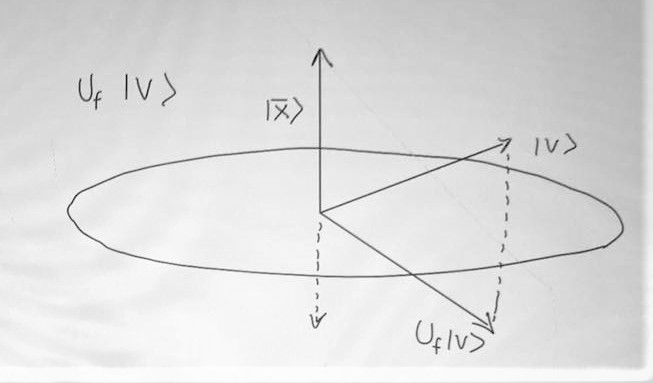
\includegraphics[width=0.7\textwidth]{Immagini/18_4/riflessione.jpg}
\caption{Interpretazione geometrica dell'azione di $U_f$ su un generico vettore $\ket{v}$\label{fig:azione-Uf}}
\end{figure}

Ciò suggerisce un'interpretazione geometrica per l'algoritmo di Grover.\\
Partiamo notando che $-R_{\ket{S}} = R_{\ket{S^\perp}}$. Infatti, un qualsiasi vettore $\ket{v}$ nell'iperpiano generato da $\{\ket{S}, \ket{S^\perp}\}$ si può scrivere come combinazione lineare:
\begin{align*}
    \ket{v} = \alpha \ket{S} + \beta \ket{S^\perp}
\end{align*}
Applicando la riflessione:
\begin{align*}
R_{\ket{S}}\ket{v} &= -\alpha \ket{S} + \beta \ket{S^\perp}\\
    R_{\ket{S^\perp}} \ket{v} &= \alpha \ket{S} - \beta \ket{S^\perp} = -R_{\ket{S}}\ket{v}\\
\end{align*}
Mettendo tutto insieme, l'algoritmo di Grover è dato da\footnote{Si ricorda che l'ordine di applicazione delle matrici è da destra a sinistra}:
\begin{align*}
    G = D U_f = R_{\ket{S^\perp}} R_{\ket{\bar{x}}}
\end{align*}

Poniamoci allora nell'iperpiano generato da $\{\ket{\bar{x}}, \ket{S}\}$ (figura \ref{fig:Grover-geom}) su cui rappresentiamo anche i vettori (unitari) perpendicolari $\ket{\bar{x}^\perp}$ e $\ket{S^\perp}$. Consideriamo uno stato iniziale $\ket{\psi}$ che appartiene al piano, e si trova ad un angolo $\alpha$ rispetto a $\ket{\bar{x}^\perp}$. Applichiamo l'algoritmo di Grover:
\begin{enumerate}
    \item L'azione dell'oracolo $U_f$ è data da $R_{\ket{\bar{x}}}$, che inverte la componente di $\ket{\psi}$ lungo $\ket{\bar{x}}$ (riflessione rispetto a $\ket{\bar{x}^\perp}$).
    \item L'azione di $D$ è la riflessione $R_{\ket{S^\perp}}$, che porta $U_f \ket{\psi}$ a $G\ket{\psi}$, riflettendolo rispetto a $\ket{S}$.
\end{enumerate}
Detto $\beta$ l'angolo tra $\ket{S}$ e $G\ket{\psi}$, l'angolo tra $U_f \ket{\psi}$ e $G\ket{\psi}$ è $2\beta$, o equivalentemente a $\beta + \theta + \alpha$:
\begin{align*}
    2\beta = \beta + \theta + \alpha \Rightarrow \beta = \theta + \alpha
\end{align*}
L'angolo tra $\ket{\psi}$ e $G\ket{\psi}$ è pari a $2\beta - 2\alpha$, ossia a $2\theta$. Perciò l'azione di $D$ corrisponde ad una rotazione di $\ket{\psi}$ di un angolo $2\theta$.

\begin{figure}[H]
\centering
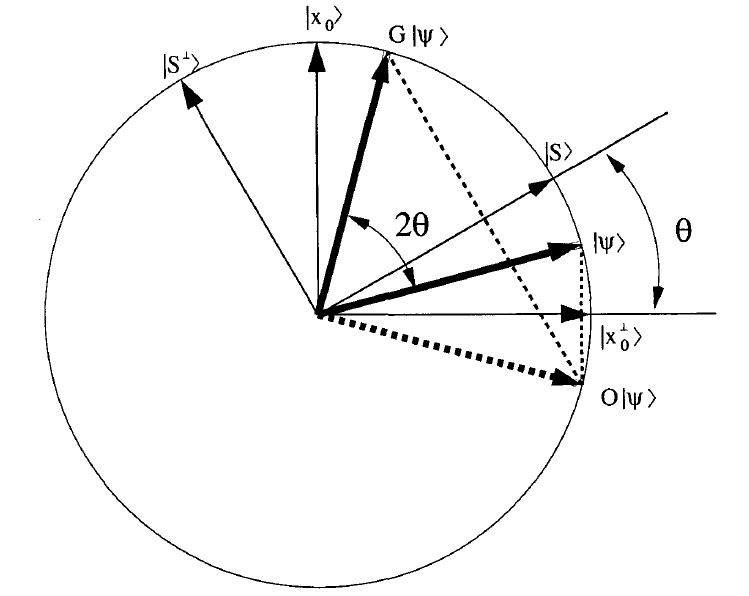
\includegraphics[width=0.7\textwidth]{Immagini/18_4/Grover_geom.PNG}
\caption{Interpretazione grafica dell'algoritmo di Grover.\label{fig:Grover-geom}}
\end{figure}

Poiché lo stato iniziale $\ket{\psi_0}$ è pari a $\ket{S}$ (è la sovrapposizione creata dalle due Hadamard iniziali) si ha:
\begin{align*}
    \ket{\psi_0} = \ket{S} = \sin\theta \ket{\bar{x}} + \cos\theta \ket{\bar{x}^\perp}
\end{align*}
dato che $\theta$ è, per definizione, l'angolo tra $\ket{S}$ e $\ket{\bar{x}^\perp}$. Poiché stiamo lavorando con $2$ soli qubit, possiamo calcolare direttamente $\theta$:
\begin{align*}
    \cos\left(\frac{\pi}{2}-\theta\right) = \sin\theta = \braket{S|\bar{x}} = \frac{1}{\sqrt{2^2}} = \frac{1}{2} \Rightarrow \theta = 30^\circ
\end{align*}
per qualsiasi scelta di $\bar{x}$, dato che $\ket{S}$ le comprende tutte con ugual probabilità.\\
Ma allora, dopo una rotazione di $2\theta = 60^\circ$, il vettore $D\ket{S}$ ha un angolo $\theta = 90^\circ$ rispetto a $\ket{\bar{x}^\perp}$, e quindi $D\ket{S} = \ket{\bar{x}}$ - esattamente come previsto dal calcolo matriciale.\\

Notiamo allora che tutti i ragionamenti fatti possono essere \textbf{generalizzati}\marginpar{Generalizzazione a $n$ qubit} al caso di indici con $n$ qubit, applicando $n$ Hadamard ai primi $n$ qubit (il ruolo dell'ancilla resta invariato):
\begin{align*}
    \ket{\Psi_1} = H^{\otimes n} \ket{0\cdots 0}_n = \frac{1}{\sqrt{2^n}} \sum_{x=0}^{2^n-1} \ket{x}_n \equiv \ket{S}
\end{align*}
In tal caso, tuttavia, l'angolo $\theta_0$ di partenza (ossia quello tra $\ket{S}$ e $\ket{\bar{x}^\perp}$) è dato da:
\begin{align*}
    \sin\theta_0 = \frac{1}{\sqrt{2^n}} \leq \frac{1}{2} \Rightarrow \theta_0 \leq 30^\circ
\end{align*}
Dopo l'applicazione dell'algoritmo di Grover, $\ket{\Psi_1}$ viene ruotato di $2\theta$ verso $\bar{x}$, ma per $n>2$ ciò non è sufficiente a far sì che $\ket{\Psi_1} = \ket{\bar{x}}$. Risulta quindi necessario \textbf{ripetere} più volte l'algoritmo. In generale, dopo $j$ ripetizioni di $G$ lo stato del sistema è:
\begin{align}
    \ket{\Psi_j} \equiv G^j \ket{S} = \sin((2j+1)\theta)\ket{x_0} + \cos((2j+1)\theta)\ket{\bar{x}^\perp}
    \label{eqn:Gj}
\end{align}
Possiamo fermare l'algoritmo dopo un certo numero $k$ di passi per cui:
\begin{align*}
    (2k+1)\theta \approx \frac{\pi}{2}
\end{align*}
ossia tale che $\ket{\psi_k} \approx \ket{\bar{x}}$. Invertendo la relazione si trova:
\begin{align*}
    k = \left \lfloor \frac{\pi}{4\theta} - \frac{1}{2} \right \rceil 
\end{align*}
dove $\lfloor \cdots \rceil$ indica l'arrotondamento all'intero più vicino (poiché chiaramente non si può effettuare un numero frazionario di passi).\\
Per $n$ sufficientemente grande:
\begin{align*}
    \sin \theta = \braket{S|\bar{x}} = \frac{1}{\sqrt{2^n}} \Rightarrow \theta \approx \frac{1}{\sqrt{2^n}} \Rightarrow k=\left \lfloor \frac{\pi}{4} \sqrt{N} - \frac{1}{2} \right \rceil = O(\sqrt{N})
\end{align*}
dove $N=2^n$ è la dimensione del database.\\

\begin{expl}\textbf{Possibilità di errore}. Lo stato finale, prodotto dall'algoritmo di Grover dopo $k$ passaggi, è molto vicino alla soluzione, ma non coincide con essa. Vi è quindi una certa probabilità $p_{\op{fail}}$ che la misura finale non risulti nel valore desiderato $\bar{x}$. Dimostriamo ora che $p_{\op{fail}}$ decade come $1/N$, ed è perciò in genere trascurabile.\\
$p_{\op{fail}}$ è pari al modulo quadro del coefficiente di $\ket{\bar{x}^\perp}$ in (\ref{eqn:Gj}) dopo $k$ iterazioni di $G$:
\begin{align}
    p_{\op{fail}} = \left|\cos \left( (2k+1)\theta \right) \right|^2 
    \label{eqn:pfail}
\end{align}
Per $N\gg 1$ si ha:
\begin{align*}
    k = \left \lfloor \frac{\pi}{4}\sqrt{N} - \frac{1}{2}\right \rceil \approx \frac{\pi}{4}\sqrt{N}; \qquad \theta \approx \frac{1}{\sqrt{N}}
\end{align*}
Sostituendo in (\ref{eqn:pfail}) giungiamo a:
\begin{align*}
    p_{\op{fail}} \approx \left | \cos \left( \frac{\pi}{2} + \frac{1}{\sqrt{N}} \right) \right|^2 \underset{(a)}{\approx} \left|\frac{\pi}{2}- \left(\frac{\pi}{2}-\frac{1}{\sqrt{N}}\right) \right|^2 = \frac{1}{N}
\end{align*}
dove in (a) si è usata l'espansione di $\cos(x)$ attorno a $x=\pi/2$:
\begin{align*}
    \cos(x) \underset{x\approx \pi/2}{=} \left( \frac{\pi}{2}-x\right) + O\left(x - \frac{\pi}{2}\right)^3
\end{align*}
\end{expl}

Al giorno d'oggi, tuttavia, l'algoritmo di Grover è solo una \textit{proof of concept}. Il problema è implementare fisicamente l'oracolo $U_f$. L'idea è che $U_f$ è determinata dal database in questione e della stringa cercata. Non esistendo un sistema generale per \q{convertire} un database classico e una stringa da cercare in un'implementazione quantistica di $U_f$, l'algoritmo di Grover non è facile da utilizzare.\\
Del resto, è possibile che l'implementazione fisica di $U_f$ vari drasticamente a seconda della stringa cercata - e perciò risulti realizzabile solo \q{sapendo a priori la soluzione}, cosa che ne rimuove l'utilità pratica. Un altro problema è immagazzinare le entrate del database in una memoria quantistica - cosa che richiede di manipolare molti più qubit di quanto non sia possibile fare al giorno d'oggi.

\section{Quantum Fourier Transform}
Si può rappresentare una stringa di (qu)bit come combinazione lineare di una certa base di stringhe - la base \textit{di Fourier}. Esplicitamente, data una sequenza di $N$ termini complessi $\{f(0), f(1), \dots, f(N-1)\}$, la \textbf{trasformata di Fourier discreta} è una nuova sequenza di $N$ numeri complessi $\{\tilde{f}(0), \tilde{f}(1), \dots, \tilde{f}(N_1)\}$ dati da:
\begin{align}
    \tilde{f}(k) = \frac{1}{\sqrt{N}} \sum_{j=0}^{N-1} \exp\left( \frac{2\pi i}{N} jk \right) f(j)
    \label{eqn:cft}
\end{align}
Tale formula - a meno di fattori di normalizzazione convenzionali - non è altro che una versione \textit{discreta} della trasformata di Fourier di una funzione.\\

Poiché si tratta di un operatore unitario, è possibile adattarla direttamente al caso di un registro di $n$ qubit ($N=2^n$):
\begin{align}
\op{QFT}(\ket{j}) = \frac{1}{\sqrt{N}} \sum_{k=0}^{N-1} \exp\left(2\pi i \frac{jk}{N}\right) \ket{k} \quad \forall \ket{j} \in \bb{C}^N
\label{eqn:QFT1}
\end{align}

Ricaviamo un'espressione in termini di gate quantistici per la QFT.\\
Partiamo scrivendo $k$ in rappresentazione binaria:
\begin{align*}
k = k_{n-1} 2^{n-1} + \dots + k_0 2^0 = \sum_{t=0}^{n-1} k_t 2^t
\end{align*}
dove $k_i$ è l'$i$-esima cifra, con $i=0$ che corrisponde alla cifra meno significativa (LSB) e $i=n-1$ a quella più significativa (MSB).\\
Sostituendo in (\ref{eqn:QFT1}), scomponiamo la somma tra $k=0$ e $k=N-1$ in una serie di $n$ somme annidate su ciascun bit:
\begin{align} \label{eqn:QFT-2}
    \op{QFT}(\ket{j}) &= \frac{1}{\sqrt{N}} \sum_{k_{n-1}=0}^1 \cdots \sum_{k_0=0}^1
    \exp\left( \frac{2\pi i j}{2^n} \sum_{t=0}^{n-1} 2^l k_l \right) \ket{k_{n-1} \cdots k_0}
\end{align}
Manipoliamo la sommatoria all'interno dell'esponenziale:
\begin{align*}
    \sum_{t=0}^{n-1} \frac{2^t k_t}{2^n} = \sum_{t=0}^{n-1} \frac{k_t}{2^{n-t}} \underset{(a)}{=} \sum_{l=1}^n \frac{k_{n-l}}{2^l}
\end{align*}
dove in (a) scegliamo di usare come indice della sommatoria l'esponente del $2$ al denominatore, ponendo $l = n-t$, da cui $t=n-l$, cosa che permetterà ad un passaggio successivo di introdurre la notazione binaria frazionale. Quando $t=0$ si ha $l=n$, mentre quando $t=n-1$, $l=n-(n-1) = 1$, e perciò i nuovi estremi sono $l=1$ e $l=n$. Nel sostituire in (\ref{eqn:QFT-2}) trasformiamo una sommatoria ad esponente in un prodotto di esponenziali:
\begin{align*}
    \op{QFT}(\ket{j}) &= \frac{1}{\sqrt{N}} \sum_{k_{n-1}=0}^1 \cdots \sum_{k_0=0}^1 \left [ \prod_{l=1}^n \exp\left( 2\pi i j \frac{k_{n-l}}{2^l}\right) \right ]
    \ket{k_{n-1} \cdots k_0}
\intertext{Notando che:}
\span \ket{k_{n-1} \cdots k_0} = \bigotimes_{l=1}^n \ket{k_{n-l}}
\intertext{Possiamo riscrivere:}
    \op{QFT}(\ket{j}) &= \frac{1}{\sqrt{N}} \sum_{k_{n-1}=0}^1 \cdots \sum_{k_0=0}^1 \bigotimes_{l=1}^n \exp\left( 2\pi i j \frac{k_{n-l}}{2^l}\right)
    \ket{k_{n-l}}
\intertext{Analogamente, le sommatorie annidate non sono altro che un prodotto di sommatorie, per cui:}
    \op{QFT}(\ket{j}) &= \frac{1}{\sqrt{N}} \bigotimes_{l=1}^n \left[
    \sum_{k_{n-l}=0}^1 \exp\left( 2\pi i j \frac{k_{n-l}}{2^l} \right) \ket{k_{n-l}}
    \right ]
\intertext{Non resta che svolgere esplicitamente l'unica sommatoria rimasta:}
    &= \frac{1}{\sqrt{N}} \bigotimes_{l=1}^n \left[
    \ket{0} + \exp\left( 2\pi i j \frac{1}{2^l}\right) \ket{1}
    \right ]
\end{align*}
Scriviamo infine $j$ in notazione binaria:
\begin{align*}
    j = j_{n-1}j_{n-2}\dots j_0 = \sum_{t=0}^{n-1} j_t 2^t
\end{align*}
e introduciamo la notazione binaria frazionale:
\begin{align*}
    0.j_l j_{l+1} \dots j_m = \frac{1}{2} j_l + \frac{1}{4} j_{l+1} + \dots + \frac{1}{2^{m-l+1}} j_m
\end{align*}
In questo modo possiamo calcolare $j/2^l$:
\begin{align*}
    \frac{j}{2^l} = j_{n-1} j_{n-2} \dots j_{l+1}.j_l \dots j_0
\end{align*}
Fattorizzando l'esponenziale, notiamo che la parte \textbf{intera} non è importante:
\begin{align*}
    \exp\left(2\pi i\frac{j}{2^l} \right) = \underbrace{\exp\left( 2\pi i j_{n-1}\dots j_{l+1} \right)}_{=1} \exp\left( 2\pi i 0.j_l \dots j_0 \right)
\end{align*}
Possiamo così espandere il prodotto tensore:
\begin{align}
    \op{QFT}(\ket{j}) &= \frac{1}{\sqrt{N}} \Big[ \ket{0} + \exp(2\pi i 0.j_0) \ket{1}\Big]_{n-1} \otimes \Big[\ket{0} + \exp(2\pi i 0.j_1 j_0 ) \ket{1}\Big]_{n-2} \otimes \cdots \otimes \\
    &\qquad \otimes\Big[\ket{0} + \exp(2\pi i 0.j_{n-1} j_{n-2}\dots j_0)\ket{1} \Big]_0 
    \label{eqn:QFT-f}
\end{align}

Notiamo che gli stati dei singoli qubit sono ancora separabili: in altre parole, la QFT non produce \textit{entanglement}.\\

L'espressione (\ref{eqn:QFT-f}) può essere ora realizzata mediante gate elementari.\\ Partiamo notando che l'$n-1$-esimo qubit della trasformata dipende solo dallo stato del primo qubit - $\ket{j_0}$ - e può essere ottenuto mediante un'Hadamard:
\begin{align*}
    \op{QFT}(\ket{j})_{n-1} \equiv \ket{\tilde{j}}_{n-1} = \frac{1}{\sqrt{2}}\Big[\ket{0} + \exp(2\pi i 0.j_0) \ket{1} \Big] = H\ket{j_0}
\end{align*}
Infatti, $j_0$ può essere $1$ o $0$:
\begin{align*}
    j_0 = 0: \qquad \ket{\tilde{j}}_{n-1} &= \frac{1}{\sqrt{2}}\Big[\ket{0} + \ket{1}\Big] = H\ket{0}\\
    j_1 = 0: \qquad \ket{\tilde{j}}_{n-1} &= \frac{1}{\sqrt{2}}\Big[\ket{0} + \exp(\pi i) \ket{1}\Big] = \frac{1}{\sqrt{2}}\Big[\ket{0}-\ket{1}\Big] = H\ket{1}
\end{align*}
Il qubit successivo, l'$n-2$-esimo, ha una fase più complessa. La parte $0.j_1$ si può ottenere applicando un'Hadamard a $\ket{j_1}$, ma resta un contributo $0.0j_0$ che richiede una C-PHASE controllata da $\ket{k_0}$. Definiamo, in generale, la C-PHASE di ordine $k$ come:
\begin{align*}
R_k = \begin{pmatrix} \bb{I}_2 & \bb{O}\\
\bb{O} & R_z(2\pi i/2^k) \end{pmatrix}
\end{align*}
Ne risulta che lo stato del qubit $n-2$-esimo è dato da:
\begin{align*}
    \ket{\tilde{j}}_{n-2} = R_2^{\ket{j_0}} H \ket{j_1}
\end{align*}
Generalizzando, per $m\geq 1$:
\begin{align*}
    \ket{\tilde{j}}_{m} = R_{m+1}^{\ket{j_0}} \cdots R_3^{\ket{j_{m-2}}} R_2^{\ket{j_{m-1}}} H \ket{j_m} = \left(\prod_{l=0}^{m-1} R_{m+1-l}^{\ket{j_l}} \right) H \ket{j_m}
\end{align*}
Mettendo tutto insieme si ottiene il circuito rappresentato in figura \ref{fig:QFT-gates}. Si noti che l'ordine dei qubit dopo la QFT è invertito. Ciò può essere corretto con un'operazione di SWAP (di ordine $O(N)$), oppure semplicemente \textit{rinominando} i qubit.

\begin{figure}[H]
    \centering
    \begin{tikzpicture}
    \node[scale=0.9] {
    \begin{quantikz}[column sep=0.1cm]
        \lstick{$\ket{j_{n-1}}$} & \gate{H} & \gate{R_2} & \ \ldots \ \qw &  \gate{R_{n-1}} & \gate{R_n} & \qw & \qw & \qw & \qw &
        \rstick{$\ket{\tilde{j}_0} = \ket{0} + \exp(2\pi i 0.j_{n-1}j_{n-2}\dots j_0)\ket{1}$} \qw \\
        \lstick{$\ket{j_{n-2}}$} & \qw & \ctrl{-1} & \ \ldots \ \qw & \qw & \qw & \gate{H} & \ \ldots \ \qw & \gate{R_{n-2}} & \gate{R_{n-1}} & \rstick{$\ket{\tilde{j}_{1}} = \ket{0} + \exp(2\pi i 0.j_{n-2}\dots j_0)\ket{1}$} \qw \\
        \wave&&&&&&&&&&&&&\\
        \lstick{$\ket{j_1}$} & \qw & \qw & \qw & \ctrl{-3} & \qw & \qw & \qw & \ctrl{-2} & \qw & \ \ldots \ \qw & \gate{H} & \gate{R_2} & \qw\\
        \lstick{$\ket{j_0}$} & \qw & \qw & \qw & \qw & \ctrl{-4} & \qw & \qw & \qw & \ctrl{-3} & \ \ldots \ \qw & \qw & \ctrl{-1} & \gate{H} & \rstick{$\ket{\tilde{j}_{n-1}} = \ket{0} + \exp(2\pi i 0.j_0)\ket{1}$}
    \end{quantikz}
    };
    \end{tikzpicture}
    \caption{Schema a porte logiche per la QFT\label{fig:QFT-gates}}
\end{figure}

In totale stiamo usando $n^2$ porte logiche quantistiche, e perciò l'algoritmo è di ordine $O(n^2)$. Classicamente, l'ordine di una trasformata discreta è $O(N^2)$, e quello dell'implementazione più efficiente (FFT, Fast Fourier Transform) è $O(Nn)$. A prima vista, perciò, il guadagno quantistico sembrerebbe esponenziale. Va però ricordato che per estrarre l'informazione necessaria dallo stato finale sarà necessario fare misure di tomografia quantistica (per determinare le fasi relative), il cui numero cresce esponenzialmente con $n$. Ne risulta che, in sé, la QFT non offre particolari vantaggi. 

\section{Computer quantistici e crittografia classica}
La trasformata di Fourier quantistica può però essere utilizzata all'interno di algoritmi quantistici più complessi - e in questo caso permette di ottenere dei \textit{guadagni computazionali}.\\

In particolare, l'algoritmo di Shor permette di fattorizzare in maniera efficiente numeri primi. Ciò è estremamente utile, dato che permette di \textit{violare} con maggiore facilità l'algoritmo (classico) di crittografia a chiave pubblica.

\subsection{La crittografia RSA}
Introduciamo una nuova tipologia di crittografia, detta \textbf{asimmetrica}. Creiamo due \textbf{chiavi}, una pubblica $\pi$ e una privata $k$. La prima è necessaria per \textit{criptare} il messaggio, la seconda per \textit{decrittarlo}:
\begin{align*}
E_\pi (P) = C; \qquad D_k(C) = P
\end{align*}
L'idea è che solo sapendo la chiave privata si possa decrittare il messaggio. Perciò la chiave pubblica può essere distribuita pubblicamente senza compromettere la sicurezza dei messaggi cifrati.\\
Ciò permette di risolvere (classicamente) il problema dello \textit{scambio delle chiavi}. Consideriamo il seguente protocollo:
\begin{enumerate}
\item Bob crea $\pi$ e $k$, e trasmette la chiave pubblica $\pi$ ad Alice
\item Alice usa $\pi$ per crittografare un messaggio: $E_\pi (P) = C$. Alice passa ora $C$ a Bob.
\item Bob è l'unico che può decrittare il messaggio $C$, dato che è l'unico in possesso della chiave privata $k$, che non è mai stata inviata a nessuno:
\begin{align*}
D_k(C) = P
\end{align*}
\end{enumerate}

L'algoritmo RSA, alla base delle tecnologie moderne di sicurezza informatica (per esempio le connessioni sicure SSH), si basa sul modello di crittografia asimmetrica.

\begin{expl}
\textbf{Costruzione dell'algoritmo RSA}. L'idea alla base di RSA sta nell'uso di \textit{one-way functions}, ossia funzioni che sono \textit{facili} da calcolare, ma molto \textit{difficili} (in senso di complessità algoritmica) da invertire. Una funzione di questo tipo è l'\textbf{esponenziale modulare}. Un numero $P$ viene elevato a un numero intero $e$, e poi diviso per un altro intero $N$. Il risultato è il \textit{resto} di tale divisione intera:
\begin{align*}
    P^e \mod N = C
\end{align*}
Si ha immediatamente $0\leq C < P$. Questo è il passaggio di \textit{codifica}, e la coppia $(N,e)$ costituisce la \textbf{chiave pubblica}.\\
La funzione inversa dell'esponenziale modulare, detta \textit{logaritmo discreto modulare} è molto difficile da computare. Cerchiamo ora una \textit{trapdoor}, ossia un'informazione aggiuntiva che - se conosciuta - rende immediata l'inversione. Tale \textit{trapdoor} costituirà la \textbf{chiave privata}, in possesso dell'unica persona che può decifrare $C$.\\
Consideriamo allora un intero $d$ che \textit{realizzi l'inversione}, ossia che:
\begin{align*}
    C^d \mod N = m
\end{align*}
Unendo le due equazioni, ciò equivale a:
\begin{align}
    P^{ed} \mod N = P
    \label{eqn:Ped}
\end{align}
Ci serve un modo per scegliere $e$, $d$ ed $N$ in modo che la trapdoor $d$ sia \textit{difficile} da ricavare conoscendo solo $N$ ed $e$. Ciò è realizzato da una seconda \textit{one-way function}, scelta per le sue proprietà in relazione all'esponenziale modulare.\\
L'idea è di sfruttare il problema della fattorizzazione in numeri primi. Mentre è facile calcolare $N=p_1 p_2$, con $p_1$, $p_2$ primi, è molto più difficile trovare i fattori conoscendo solo $N$.\\
Consideriamo ora la funzione $\varphi(n)$ (detta anche $\varphi$ di Eulero, o \textit{toziente}), che associa ad un numero $n$ il numero di interi compresi tra $1$ e $n$ che sono coprimi con $n$. Per esempio, per $n=8$, solo $1,3,5,7$ sono $\leq 8$ e non condividono fattori con $8$ (eccetto $1$), e perciò $\varphi(8)=4$. In generale, $\varphi(n)$ è difficile da calcolare - eccetto nel caso in cui $n$ sia primo, in cui semplicemente $\varphi(n) = n-1$. Di più, poiché $\varphi$ è moltiplicativa, ossia $\varphi(ab) = \varphi(a) \varphi(b)$, per $p_1$, $p_2$ primi vale:
\begin{align*}
    \varphi(p_1 p_2) = \varphi(p_1)\varphi(p_2)=(p_1-1)(p_2-1)
\end{align*}
Possiamo mettere tutto insieme utilizzando il \textbf{teorema di Eulero} (che generalizza il piccolo teorema di Fermat):
\begin{align*}
    P^{\varphi(n)} \equiv 1 \mod n
\end{align*}
Elevando entrambi i membri ad un intero $k$, poiché $1^k = 1$, vale:
\begin{align*}
    P^{k\varphi(n)} \equiv 1 \mod n
\end{align*}
Moltiplicando per $P$:
\begin{align*}
    P^{k\varphi(n)+1} \equiv P \mod n
\end{align*}
Confrontando con (\ref{eqn:Ped}) troviamo allora:
\begin{align*}
    k\varphi(n)+1 = ed \Rightarrow d = \frac{k\varphi(n)+1}{e}
\end{align*}
Scegliendo $n=p_1 p_2$, con $p_1$, $p_2$ primi, solo conoscendo i fattori (difficili da ricavare sapendo solo $N$) possiamo calcolare facilmente $\varphi(n)$, e di conseguenza $d$ - che funge da \textit{trapdoor}. Del resto, $k$ è scelto per far sì che $d$ sia intero, mentre per $e$ si può prendere un qualche numero $1< e < \phi(n)$ coprimo con $\varphi(n)$).
\end{expl}

Esaminiamo i passaggi dell'algoritmo.
\begin{enumerate}
\item Bob crea un numero $N$ dato dal prodotto $p\cdot q$ di due numeri \textbf{primi} $p,q$ sufficientemente grandi. Mentre generare numeri primi e moltiplicarli tra loro è efficiente, \textit{fattorizzare} un numero grande in numeri primi è computazionalmente molto costoso. Perciò possiamo essere sicuri che, se uno sa solo $N$, non sarà in grado di ottenere $p$ e $q$ con facilità (il processo potrebbe richiedere con i computer odierni tempi di milioni di anni).\\
Bob calcola anche:
\begin{align*}
\Phi = (p-1)(q-1)
\end{align*}
Inoltre sceglie un numero $1<e<\Phi$ che sia \textit{coprimo} con $\Phi$ (ossia che non condivide fattori $\neq 1$ con $\Phi$) e infine calcola $d$ tale che $d\cdot e = 1 \mod \Phi$.\\
Tale $d$ costituisce la \textbf{chiave privata}, mentre la coppia di numeri $(e,N)$ è la \textbf{chiave pubblica} che viene passata ad Alice.
\item Alice, conoscendo $(e,N)$, può codificare messaggi nel seguente modo. Il messaggio da inviare \footnote{Generalmente RSA si usa per inviare in modo sicuro le chiavi di altri algoritmi a cifratura simmetrica, che hanno il vantaggio di essere molto più veloci.} è codificato in una stringa di bit, ossia un numero $P$, e supponiamo che sia $P< N$. Allora il messaggio cifrato $C$ si calcola come:
\begin{align}
C = E_\pi (P) = P^e \mod N \label{eqn:crittoRSA}
\end{align}
Alice invia poi $C$ a Bob.
\item Bob ha ora tutte le informazioni necessarie per decodificare $C$:
\begin{align}
P = D_k(C) = C^d \mod N
\label{eqn:decritt}
\end{align}
\end{enumerate}

\textbf{Dimostrazione}.
Vogliamo dimostrare (\ref{eqn:decritt}). Inserendo (\ref{eqn:crittoRSA}), ciò equivale a:
\begin{align}
C^d \mod N = P^{ed} \mod N \overset{?}{=} P
\label{eqn:C-d}
\end{align}
e ciò deve valere $\forall P$.\\
Sappiamo che $p \neq q$ sono numeri primi, e che $e$, $d$ sono numeri naturali tali che $ed \equiv 1 \mod \Phi$. Per definizione di modulo, $\exists k \in \bb{N}$ tale che:
\begin{align*}
    ed = k\Phi + 1 \underset{(a)}{=} k(p-1)(q-1) + 1
\end{align*}
dove in (a) si è usato $\phi = (p-1)(q-1)$. Riarrangiando:
\begin{align*}
    ed - 1 = k(p-1)(q-1)
\end{align*}
ossia $ed-1$ è multiplo sia di $(p-1)$ che di $(q-1)$. Esplicitamente:
\begin{align}
    \label{eqn:multipli}
    \exists h,j \in \bb{N} \mid ed-1 = h(p-1) = j(q-1)
\end{align}
Poiché $p$ e $q$ sono primi, possiamo spezzare l'uguaglianza da verificare in due:
\begin{align*}
    P^{ed} \mod pq \equiv P \Leftrightarrow \begin{cases}
    P^{ed} \mod p \equiv P\\
    P^{ed} \mod q \equiv P
    \end{cases}
\end{align*}
\begin{itemize}
    \item Partiamo dal $\op{mod} p$. Se $P\equiv 0 \mod p$, segue immediatamente che $P^{ed}$ è multiplo di $p$, e quindi anche $P^{ed} \equiv 0 \equiv P \mod p$. Generalmente, però, $P \not\equiv 0$. In tal caso servono alcune manipolazioni:
    \begin{align*}
        P^{ed} \mod p = P^{ed-1} P \underset{(\ref{eqn:multipli})}{=} P^{h(p-1)} P = (P^{p-1})^h P \underset{(a)}{\equiv} 1^h m \equiv m \mod p 
    \end{align*}
    dove in (a) si è usato il piccolo teorema di Fermat (che non dimostriamo), per cui:
    \begin{align*}
        P^{p-1} \equiv 1 \mod p
    \end{align*}
    
    \begin{expl}
    In effetti, ciò equivale all'enunciato del teorema di Eulero, $P^{\varphi(p)} \equiv 1 \mod p$, dato che $p$ è primo e quindi $\varphi(p)=p-1$.
    \end{expl}
    
    \item Per l'uguaglianza con $\op{mod} q$ si ripete il procedimento. Escluso il caso banale di $P\equiv 0$, avremo:
    \begin{align*}
        P^{ed} = P^{ed-1}P \underset{(\ref{eqn:multipli})}{=} P^{j(q-1)}P = (P^{q-1})^j P \equiv 1^j P \equiv P \mod q
    \end{align*}
\end{itemize}
Abbiamo allora mostrato che:
\begin{align*}
    C^d \equiv P^{ed} \equiv P \mod N
\end{align*}
e poiché $P<N$, $P\mod N = P$ $\forall P$. 
\begin{flushright}
$\square$
\end{flushright}

\end{document}

